% Chapter 1

\chapter{引言}

\section{概述}
  计算机在对一个平面形状进行栅格化时,一般需要首先将形状的曲边近似转化为折线,由此将待渲染的形状转为多边形,再将其切分为三角形并依次渲染。在切分出的三角形中,具有两个极小锐角的细长三角形被称为“sliver triangles”\upcite{edelsbrunner2000smoothing},不便于栅格化时的计算。因此,在设计多边形栅格化的算法时,常常需要在做到高效的同时避免产生细长三角形。

  本文实现了一种近似算法,可在不添加新顶点的情况下快速将任意形状带孔凹多边形划分成数个互不重合的三角形,能正确处理多种复杂情况,且产生的细长三角形数目较少,便于后续处理。
\section{研究现状}

平面多边形三角化作为计算机图形学的基础课题,当下研究较为成熟,有着较多的相关研究。近些年的论文以对已有的三角划分算法应用为主,在GIS\upcite{刘学军2001三角网数字地面模型的理论},医学图像\upcite{秦绪佳2002医学图像三维重建模型的剖切与立体视窗剪裁},计算机图形学等方面有了较多的成果。而对三角划分算法本身的研究则多发表于二十一世纪初甚至更早之前。


\section{理论基础}
三角剖分(triangulation):假设在平面有一点集V,三角形s是由点集中的点作为端点的非退化三角形,S为s的集合。则该点集V的一个三角剖分T=(V,S)是一个平面图,满足以下条件:
\begin{itemize}
  \item 平面图中的任意两个三角形交集面积为0
  \item 平面图中所有三角形的并集是点集V的凸包
\end{itemize}

Ear Clipping(耳切法)\upcite{eberly2008triangulation}是一种较为简易的多边形三角化算法,其思路简单易懂,但缺点是可能会产生较多的细长三角形。原理为不断在多边形内寻找可被切除\footnote[1]{当一个三角形内部不包含其他顶点且该三角形属于原多边形一部分时认为其可切除}的连续三个顶点构成的三角形。对于任意多边形,至少存在两个可被切除的三角形。轮流切除所有的三角形后算法结束。朴素情况下该算法的复杂度为\(O(n^2)\)。

\begin{figure}[htbp]
  \centering
  \begin{minipage}{0.4\textwidth}
      \centering
      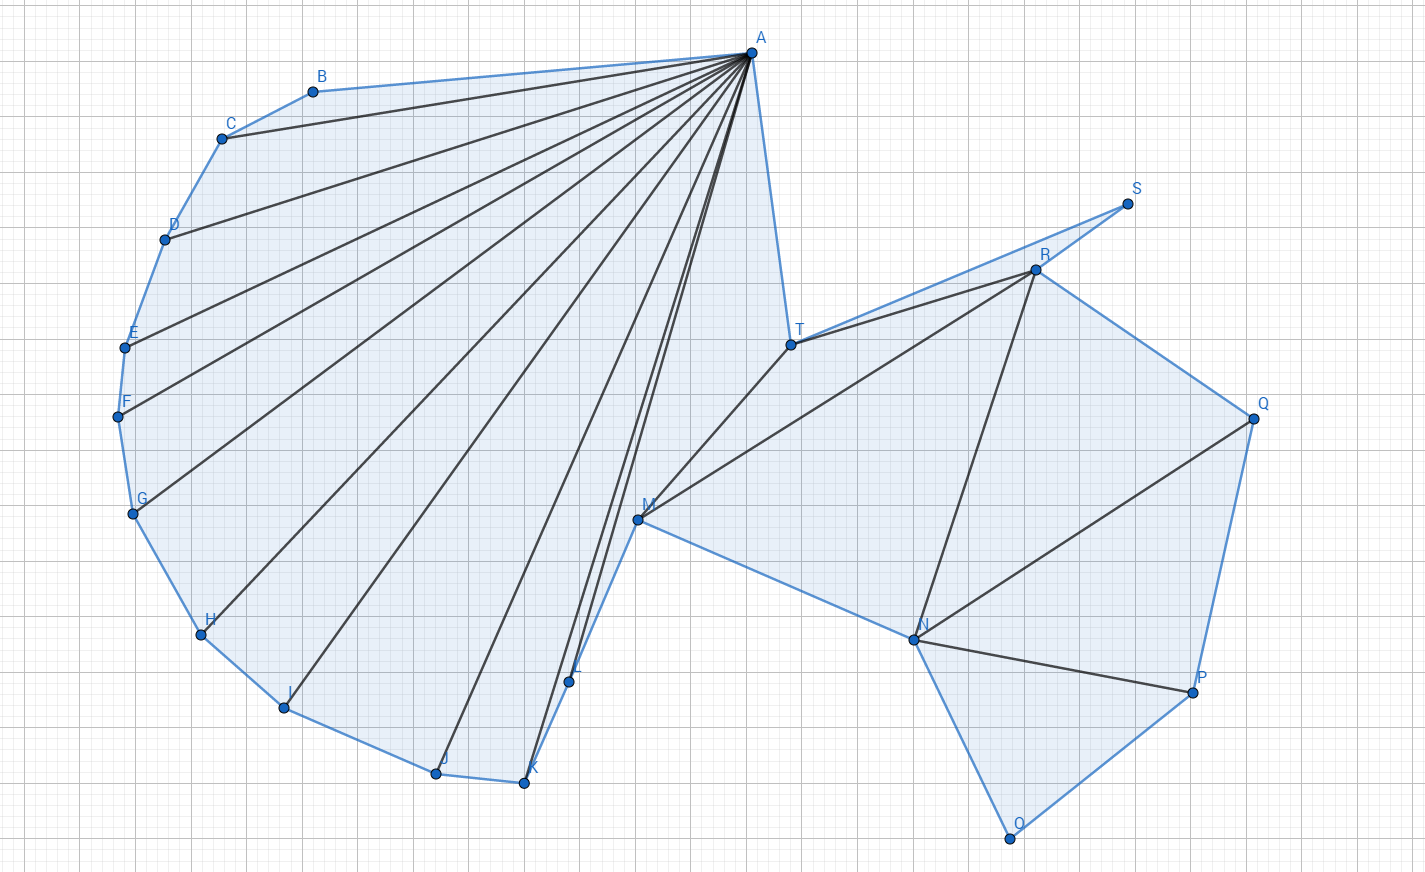
\includegraphics[width=\textwidth]
      {figures/ear clipping.png}
      \caption{耳切法的典型结果}
  \end{minipage}
  \begin{minipage}{0.4\textwidth}
      \centering
      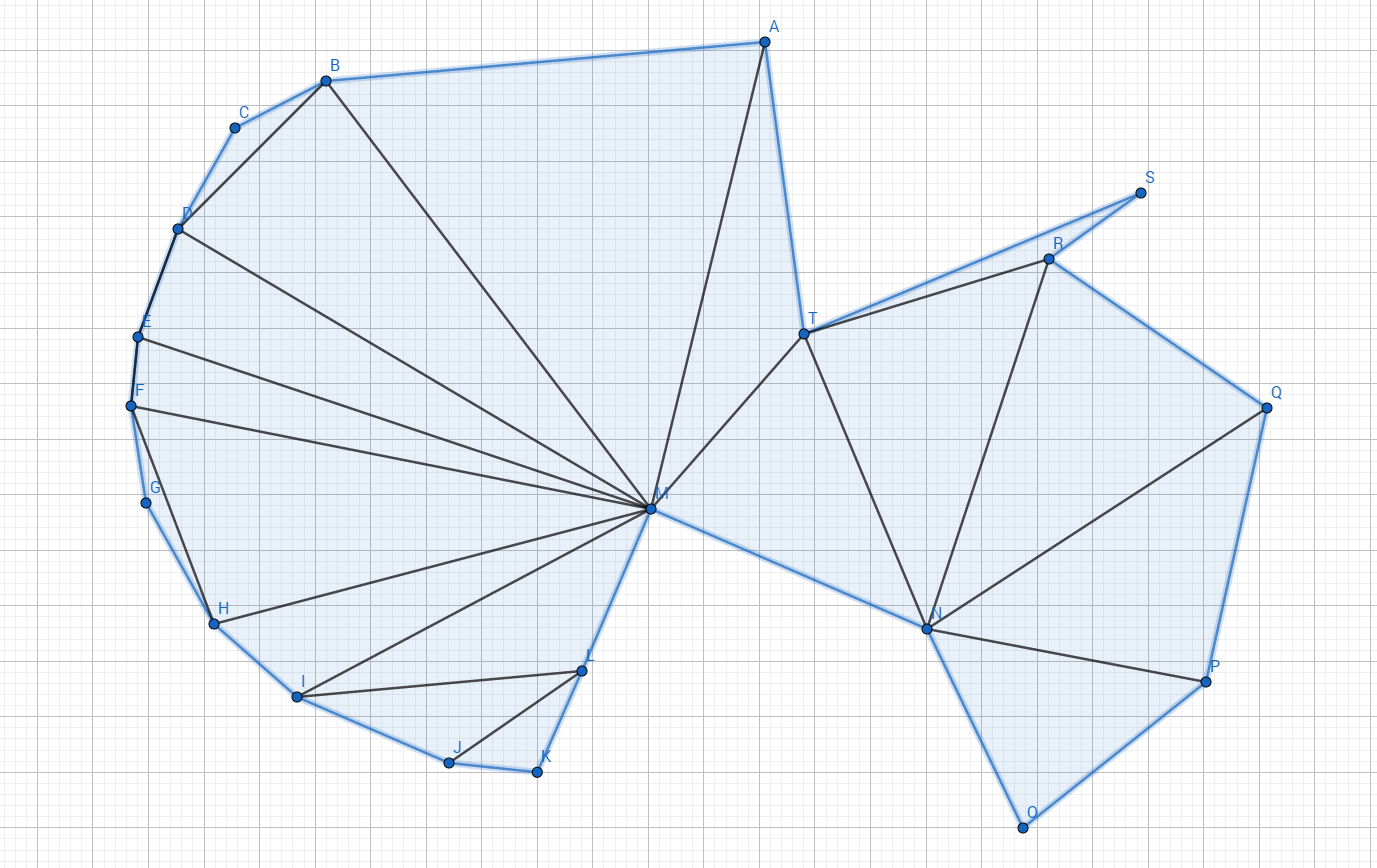
\includegraphics[width=\textwidth]
      {figures/better.png}
      \caption{相对更好的一种解}
  \end{minipage}
\end{figure}

Delaunay triangulation\upcite{闵卫东1995二维任意域内点集的Delaunay三角划分生成算法}算法则会生成一组相对更加优秀的解,其满足形成的三角形中最小角尽可能大。但该算法只适用于凸多边形的划分。虽然计算得出的解在处理后也可用于凹多边形划分,但该划分结果可能会产生新的顶点,导致最终的三角形个数增加。Delaunay三角划分有数种实现方式,其中较为常用的算法如Bowyer-Watson算法,其原理是维护一个合法的Delaunay三角划分,每次向点集中加入新点,并修改新增点附近的三角划分规则。其复杂度为\(O(n^2)\)。或者也可以采用分治法,将点集划分为两部分并合并生成的Delaunay三角划分,其时间复杂度为\(O(n*\log_2n)\)\upcite{lee1980two}。

\section{概念定义}

定义\(N_i\) 为二维平面上的点,\(N_{ix},N_{iy}\) 分别为该点的横纵坐标;

定义有序集合\(S:N_0,N_1,\cdots,N_{n-1}\)表示有n个节点的无孔洞简单多边形,对任意\(i\in [0,n-1] \)满足\(N_i,N_{(i+1) \bmod n}\)之间存在一条连边。

定义有序集合\(T:S_0,S_1,\cdots,S_{n-1}\)表示有n段边界的有孔洞简单多边形,其中\(S_0\)表示多边形的外边界,其余则表示多边形中的孔洞。

\section{代码结构}

本代码采用C++实现,在注重运行效率的同时兼顾了一定的可读性。

对于第一种算法,我们使用双向链表存储节点及其连边,每个多边形内记录一个指向链表节点的指针,整个图对象内使用数组记录指向每一个多边形的指针;

为了便于数据处理和计算,每个链表节点同时存储了当前节点的标号,部分代码处理时利用节点的标号辅助确定节点的相对位置;

图对象内同时存储了指向全部初始结点的指针,可根据需求进行排序以便于部分处理。

对于第二种算法,我们采用数组记录多边形的所有顶点,并采用链表按极角序记录每个顶点的所有连边信息。

IO部分实现了以svg图片格式输出中间过程和最终结果,可以直观的展示图片分割结果。

代码编译产物为静态链接库,可在其他程序中通过函数调用进行计算。

\section{预期效果}
代码支持从标准输入或文件读取多边形,并将分割结果以图片或三角形集合的形式输出。
多边形分割完成后由数个三角形构成,且各三角形之间互不相交,也不会产生覆盖区域在原多边形外部的三角形。
在三角剖分的结果中细长三角形的数目较少,大部分三角形较为规则。

% 与Word等所见即所得编辑工具不同,使用 \LaTeX 工具排版可以将写作与排版过程分离,写作者只需要关心文字的部分,而剩下的排版工作全部交给工具自动完成。

% \section{格式要求}
% 正文宋体小四,正文行间距固定为23磅。

% 通过空一行(两次回车)实现段落换行,仅仅是回车并不会产生新的段落。 \par

% 也可以通过 \verb|\par| 命令来新起一段。

% \section{各节一级标题}
% 我是内容

% \subsection{各节二级标题}
% 你是内容

% \subsubsection{各节三级标题}
% 他是内容

% \section{字体字号}
% {\songti \bfseries 宋体加粗} {\textbf{English}}

% {\songti \itshape 宋体斜体} {\textit{English}}

% {\songti \bfseries \itshape 宋体粗斜体} {\textbf{\textit{English}}}

% \section{编译}
% 本模板必须使用XeLaTeX + BibTeX编译,否则会直接报错。 本模板支持多个平台,结合sublime/vscode/overleaf都可以使用。